\documentclass[convert={density=1200,size=400x,outext=.png}]{standalone}
\usepackage{tikz}
\usetikzlibrary{arrows.meta,calc,shadings}
\pagestyle{empty}
\begin{document}
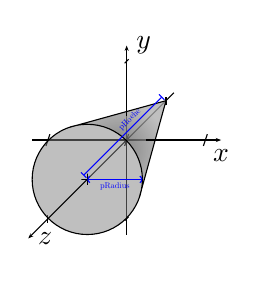
\begin{tikzpicture}[x={(1cm,0)},y={(0,1)},z={(-0.5cm,-0.5cm)},>={Stealth[scale=.4]}]
  % Achsen
  \draw (-1.2,0,0)--(.25,0,0);
  \draw (0,-1.2,0)--(0,.3,0);
  \draw (0,0,-1.2)--(0,0,1);
  % Skalenstriche
  \draw \foreach\x in {-1,...,1} { (\x,-.05,.05)--(\x,.05,-.05) };
  \draw \foreach\y in {-1,...,1} { (0,\y,-.05)--(0,\y,.05) };
  \draw \foreach\z in {-1,...,2} { (0,-.05,\z)--(0,.05,\z) };
  \fill[black!50,opacity=.5] (0,0,1) circle (.7);
  \fill[inner color=black!50,opacity=.5] (0,0,1) ++(110:.7) arc(110:-20:.7) -- (0,0,-1) -- cycle;
  \draw plot[mark=+] (0,0,1) (0,0,1) circle (.7) (0,0,1) ++(110:.7) --(0,0,-1) (0,0,1) ++(-20:.7) --(0,0,-1);
  % draw last part of the z-axis
  \draw[->] (.25,0,0)--(1.2,0,0) node[below]{$x$};
  \draw[->] (0,.3,0)--(0,1.2,0) node[right]{$y$};
  \draw[->] (0,0,1)--(0,0,2.5) node[right]{$z$};
  \draw[blue,<->, >={Parenthesis[scale=.6]}] (0,0,1)-- node[scale=.3,below]{pRadius} ++(0:.7);
  \draw[blue,<->, >={Bar[scale=.6]},shift={(-.05cm,.05cm)}] (0,0,1)--(0,0,-1) node[above,sloped,scale=.3,pos=.65] {pHoehe};
\end{tikzpicture}
\end{document}